\section{Introduction}\label{sec:intro}

The subject of this survey is a question about finite groups that began as a question about arranging officers in a square. It was answered in 2009 with the help of the classification of finite simple groups, and since then it has been answered again, twice, by purely combinatorial means. Along the way it became a question about rainbow perfect matchings, and that is the form in which most of the recent progress, and most of the open problems, are stated.

\topic{Euler's thirty-six officers}

In 1782 Euler~\cite{eul1782} posed the following problem.

\begin{problem}[Euler, 1782]\label{prob:euler}
Six regiments each send six officers, one of each of six ranks. Can the $36$ officers stand in a $6\times6$ square so that every row and every column contains one officer of each regiment and one officer of each rank?
\end{problem}

Euler found no arrangement. Smaller versions of the puzzle have solutions; a card puzzle from Ozanam's \emph{R\'ecr\'eations math\'ematiques}~\cite{oza1723} asks for the sixteen court cards to be laid out so that every row and every column contains each rank and each suit, and Figure~\ref{fig:cards} shows a solution.

\begin{figure}[ht]
\centering
\begin{tikzpicture}[every node/.style={font=\large},
      card/.style={draw, minimum size=9mm, inner sep=0pt, outer sep=0pt}]
    \def\S{$\spadesuit$}\def\C{$\clubsuit$}%
    \def\H{\textcolor{RainbowRed}{$\heartsuit$}}%
    \def\D{\textcolor{RainbowRed}{$\diamondsuit$}}%
    \foreach \i/\row in {0/{A\S,Q\C,J\H,K\D}, 1/{K\H,J\D,Q\S,A\C},
                         2/{Q\D,A\H,K\C,J\S}, 3/{J\C,K\S,A\D,Q\H}}{%
      \foreach \c [count=\j] in \row
        \node[card] at (0.9*\j, -0.9*\i) {\c};}
  \end{tikzpicture}

\caption{A solution of Ozanam's card puzzle (1723): every row and every column contains each rank and each suit.}
\label{fig:cards}
\end{figure}

Such an arrangement is two squares in one. Forgetting the suits leaves a square of ranks in which every rank occurs once in each row and each column, and forgetting the ranks leaves a square of suits with the same property (Figure~\ref{fig:card-split}). Euler wrote the regiments with Latin letters and the ranks with Greek letters, which is where the name \emph{Latin square} comes from~\cite{mon24}.

\begin{figure}[ht]
\centering
\begin{tikzpicture}[every node/.style={font=\normalsize},
      cell/.style={draw, minimum size=7mm, inner sep=0pt, outer sep=0pt}]
    \def\S{$\spadesuit$}\def\C{$\clubsuit$}%
    \def\H{\textcolor{RainbowRed}{$\heartsuit$}}%
    \def\D{\textcolor{RainbowRed}{$\diamondsuit$}}%
    % the cards
    \foreach \i/\row in {0/{A\S,Q\C,J\H,K\D}, 1/{K\H,J\D,Q\S,A\C},
                         2/{Q\D,A\H,K\C,J\S}, 3/{J\C,K\S,A\D,Q\H}}{%
      \foreach \c [count=\j] in \row
        \node[cell] at (0.7*\j, -0.7*\i) {\c};}
    \node[font=\footnotesize] at (1.75,-3.0) {the cards};
    \node at (3.75,-1.05) {$=$};
    % the ranks
    \begin{scope}[shift={(4.2,0)}]
      \foreach \i/\row in {0/{A,Q,J,K}, 1/{K,J,Q,A}, 2/{Q,A,K,J}, 3/{J,K,A,Q}}{%
        \foreach \c [count=\j] in \row
          \node[cell] at (0.7*\j, -0.7*\i) {\c};}
      \node[font=\footnotesize] at (1.75,-3.0) {the ranks};
    \end{scope}
    \node at (7.95,-1.05) {$+$};
    % the suits
    \begin{scope}[shift={(8.4,0)}]
      \foreach \i/\row in {0/{\S,\C,\H,\D}, 1/{\H,\D,\S,\C},
                           2/{\D,\H,\C,\S}, 3/{\C,\S,\D,\H}}{%
        \foreach \c [count=\j] in \row
          \node[cell] at (0.7*\j, -0.7*\i) {\c};}
      \node[font=\footnotesize] at (1.75,-3.0) {the suits};
    \end{scope}
  \end{tikzpicture}

\caption{Forgetting the suits leaves a Latin square of ranks; forgetting the ranks leaves a Latin square of suits. Every rank--suit pair occurs exactly once.}
\label{fig:card-split}
\end{figure}

\begin{definition}\label{def:latin}
A \term{Latin square} of order $n$ is an $n\times n$ array of $n$ symbols in which every symbol occurs once in each row and once in each column. Two Latin squares $A=(a_{ij})$ and $B=(b_{ij})$ of order $n$ are \term{orthogonal} if the $n^2$ pairs $(a_{ij},b_{ij})$ are all distinct.
\end{definition}

Euler's problem asks for two orthogonal Latin squares of order $6$. He conjectured that this, and more, is impossible.

\begin{conjecture}[Euler, 1782]\label{conj:euler}
For $n\equiv2\pmod4$ there are no two orthogonal Latin squares of order $n$.
\end{conjecture}

For $n=2$ this is trivially true, and Tarry~\cite{tar1900} showed in 1900 that it is true for $n=6$: the thirty-six officers cannot be arranged. Beyond that Euler was wrong. Bose and Shrikhande~\cite{bs59} found counterexamples for $n=22$ and $n=50$ in 1959, and Bose, Shrikhande and Parker~\cite{bsp60} found counterexamples for every $n\equiv2\pmod4$ with $n\geq10$ in 1960. So the conjecture holds only for $n=2$ and $n=6$.

\topic{Latin squares in field trials}

Latin squares are also a tool of experimental design. R.~A.~Fisher promoted them in his experiments at Rothamsted between 1919 and 1933 and in \emph{The Design of Experiments} (1935); see Bailey~\cite{bai13}. The reason for balancing rows \emph{and} columns is the shape of a field. In Fisher's words, quoted by Bailey, ``on any given field agricultural operations \dots\ have followed one of two directions \dots; consequently streaks of fertility, weed infestation, etc., do, in fact, occur predominantly in those two directions'' (Fisher to Jeffreys, 1938). The oldest known example, again from Bailey, is an experiment on sixteen sheep by Cretté de Palluel in 1790 (Figure~\ref{fig:sheep}): the rows are slaughter dates, the columns are breeds, and the entries are diets, each diet occurring once on each date and once in each breed.

\begin{figure}[ht]
\centering
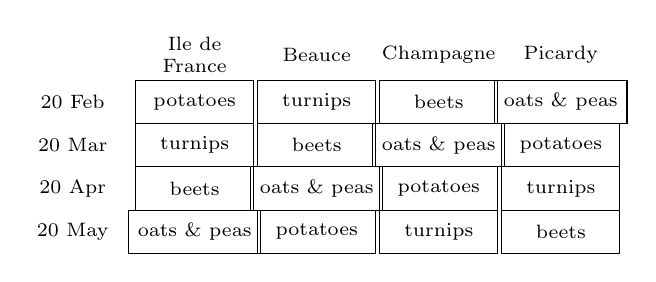
\begin{tikzpicture}[every node/.style={font=\scriptsize}]
    \foreach \b [count=\j] in {Ile de France,Beauce,Champagne,Picardy}
      \node[align=center, text width=1.45cm] at (1.55*\j,0.05) {\b};
    \foreach \d [count=\i] in {20 Feb,20 Mar,20 Apr,20 May}
      \node at (0,-0.55*\i) {\d};
    \foreach \row [count=\i] in {{potatoes,turnips,beets,oats \& peas},
                                 {turnips,beets,oats \& peas,potatoes},
                                 {beets,oats \& peas,potatoes,turnips},
                                 {oats \& peas,potatoes,turnips,beets}}
      \foreach \c [count=\j] in \row
        \node[draw, minimum width=1.5cm, minimum height=0.55cm] at (1.55*\j,-0.55*\i) {\c};
  \end{tikzpicture}

\caption{Cretté de Palluel's experiment of 1790 on sixteen sheep~\cite{bai13}. Rows: slaughter date; columns: breed; entries: diet.}
\label{fig:sheep}
\end{figure}

Superimposing a second square orthogonal to the first balances a second family of treatments against the rows, the columns and the first family. In the statistics literature such pairs are called \term{Graeco-Latin squares}~\cite{dey17}; Euler's nine officers of three regiments and three ranks (Figure~\ref{fig:nine-officers}) are the smallest interesting example. For odd orders they are easy to write down.

\begin{figure}[ht]
\centering
\begin{tikzpicture}[every node/.style={font=\small}]
    \foreach \row [count=\i] in {{A\alpha,B\beta,C\gamma},{C\beta,A\gamma,B\alpha},{B\gamma,C\alpha,A\beta}}
      \foreach \c [count=\j] in \row
        \node[lscell, minimum size=7.5mm] at (0.75*\j,-0.75*\i) {$\c$};
  \end{tikzpicture}

\caption{Nine officers: each Latin letter meets each Greek letter exactly once~\cite{bai13}.}
\label{fig:nine-officers}
\end{figure}

\begin{proposition}[see~\cite{bai13}]\label{prop:odd-pair}
For odd $n$, the Latin squares $L_1(i,j)=i+j$ and $L_2(i,j)=i-j$ on $\Z_n$ are orthogonal.
\end{proposition}

\begin{proof}
If the cells $(i_1,j_1)$ and $(i_2,j_2)$ carry the same pair, then $i_1+j_1=i_2+j_2$ and $i_1-j_1=i_2-j_2$, so $2(j_1-j_2)=0$. As $n$ is odd, $j_1=j_2$, and then $i_1=i_2$.
\end{proof}

The square $L_1$ is the addition table of $\Z_n$, so odd cyclic groups give orthogonal pairs at once. The difficulty lies in even orders, and it is there that the structure of the group begins to matter.
